\documentclass[article,brazil,english]{techreport}

% ---
% Informações de dados para CAPA e FOLHA DE ROSTO
% ---
\titulo{Applyting the principle of superposition to the design of the magnetic circuit}
\autor{Fábio Pinto Fortkamp}
\local{Florianópolis}
\data{}
\orientador{Prof. Jader Riso Barbosa, Jr.}


% this configures PDF metadata with the above information
\configurepdf

% ---
% compila o indice
% ---
\makeindex
% ---

\usepackage{engsymbols}
\usepackage{magref}


\newcommand{\teslamax}{TeslaMax{ }}
\newcommand{\murm}{\mu_{\mathrm{r},m}}
\newcommand{\indexremmk}[2]{\mathrm{rem},{#1},{#2}}
\newcommand{\nvbremmk}[2]{\nvb_{\indexremmk{#1}{#2}}}
\newcommand{\bremmk}[2]{B_{\indexremmk{#1}{#2}}}
\newcommand{\alpharemmk}[2]{\alpha_{\indexremmk{#1}{#2}}}
\newcommand{\nvfremmk}[2]{\nvector{F}^B_{\indexremmk{#1}{#2}}}
\newcommand{\nvbiii}{\nvb\ped{III}}

% ----
% Início do documento
% ----

\graphicspath{{../figures/}}
\begin{document}

% Retira espaço extra obsoleto entre as frases.
\frenchspacing 

% ----------------------------------------------------------
% ELEMENTOS PRÉ-TEXTUAIS
% ----------------------------------------------------------
\pretextual

\maketitle

% ----------------------------------------------------------
% ELEMENTOS TEXTUAIS
% ----------------------------------------------------------
\textual

\section{Description of the \teslamax model}
\label{sec:descr-tesl-model}

The \teslamax model is the model for a novel magnetic circuit under development. Its name derive from the goal of maximizing the magnetic flux delivered to the air gap. The first quadrant of the  design can be described by \autoref{fig:teslamax}. 

\begin{figure}[!ht]
  \centering
  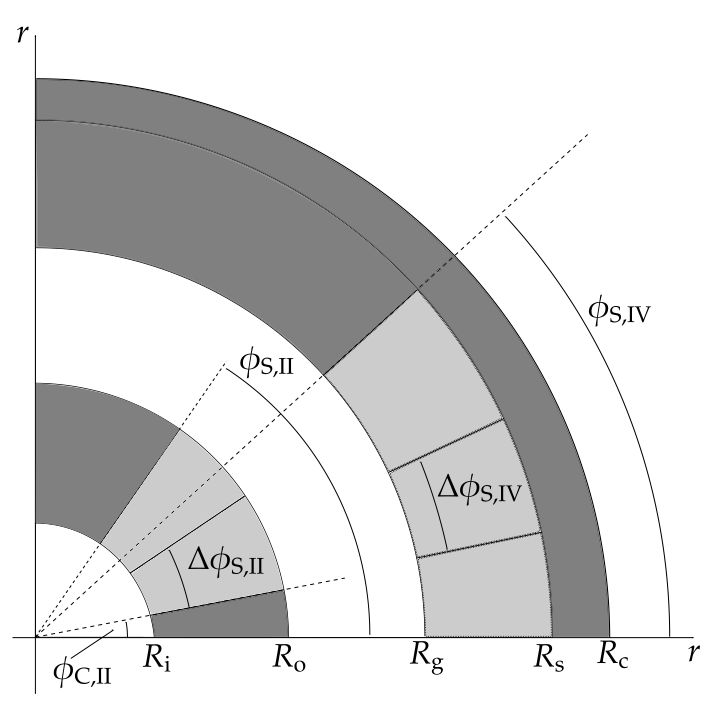
\includegraphics[width=10cm]{teslamax.pdf}
  \caption{Geometry for the \teslamax model. Dark gray areas represent iron, light gray represent permanent magnet, white represent air.}
  \label{fig:teslamax}
\end{figure}

A fundamental feature of \teslamax is that it is composed of an inner and an outer cylinder, denoted by II and IV, respectively. Each cylinder has magnet blocks of equal size (but they may be different across cylinders); there are $n\ped{II}$ blocks in the inner cylinder and $n\ped{IV}$ in the outer one. The segment numbering starts at 1 at the bottom-most unit (lowest value of the $y$-coordinate of the block's center).

All magnet segments are characterized by a relative permeability $\murm$, uniform for magnet $m$; for instance, all blocks in magnet II have permeability $\mu\ped{r,II}$. Each block is uniformily magnetized in a direction:
\begin{equation}
  \label{eq:1}
\nvbremmk{m}{k} = \bremmk{m}{k} \left( \cos\left( \alpharemmk{m}{k}  \right) \unitvector{x} + \sin\left( \alpharemmk{m}{k}  \right) \unitvector{y} \right)
\end{equation}

\noindent where $m$ represents the magnet and $k$ the segment in that magnet.


Iron blocks fill the remainder of the cylinders, and there is an iron ring outside the outer cylinder. The iron regions are characterized by a relative permeability $\mu\ped{r,iron}$ and have the purpose of guiding the flux lines.

The whole \teslamax system is linear, as will be discussed later.

Only the first quadrant is represented for simplicity; it can be shown that, to maintain a two-pole symmetry, the following conditions must be applied:

\begin{enumerate}
\item The orientation of the remanence vectors in the second quadrant is opposed to the first quadrant:

  \begin{equation}
    \label{eq:2}
    \left( \alpharemmk{m}{k}  \right)\ped{1Q} = -\left( \alpharemmk{m}{k}  \right)\ped{2Q}
  \end{equation}
\item The top half-circle (first and second quadrant) has mirror symmetry with the bottom one; this \emph{magnetic insulation} condition is equivalent to specifying:

  \begin{equation}
    \label{eq:3}
    \nvb \cdot \normalvector = 0 \quad (y = 0)
  \end{equation}
\end{enumerate}

\section{Linearity of the \teslamax model}
\label{sec:line-tesl-model}

Each region (the air gap, each magnet segment, each iron block) is governed by the following equations:

\begin{equation}
  \label{eq:4}
  \divergent{\nvb} = 0
\end{equation}

\begin{equation}
  \label{eq:5}
  \curl{\nvh} = 0
\end{equation}

\noindent and the materials follow the constitutive relation

\begin{equation}
  \label{eq:6}
  \nvb = \mur \mu_0 \nvh + \nvbrem
\end{equation}

It can be seen that, assuming the permeability is constant, all equations are linear. This is fundamental because it allows the application of the Principle of Superposition.

\section{Effect of a single magnet block}
\label{sec:effect-single-magnet}

The magnetic flux density vector field in the air gap is denoted $\nvbiii (\rvec)$.

Now imagine that only one of the blocks is magnetized (in the first quadrant; the symmetry conditions will still apply). We denote $\nvfremmk{m}{k}  (\nvbremmk{m}{k} )$ the contribution of segment $k$ in magnet $m$ to the vector field $\nvbiii$ \cite{bib:insinga16_optim}; that is, is the calculated air gap field when only this segment has its remanence $\nvbremmk{m}{k}$, with all other remanences being null.

Because of the Principle of Superposition, the vector field $\nvbiii$ can be expressed as:

\begin{equation}
  \label{eq:7}
  \nvbiii = \sum_{p=1}^{n\ped{II}} \nvfremmk{\mathrm{II}}{p} \left(\nvbremmk{\mathrm{II}}{p}\right) + \sum_{q=1}^{n\ped{IV}} \nvfremmk{\mathrm{IV}}{q} \left(\nvbremmk{\mathrm{IV}}{q}\right)
\end{equation}

Also because of the linearity, \autoref{eq:1} can be inserted into \autoref{eq:7} to give:

\begin{equation}
\begin{split}
    \nvbiii = &\sum_{p=1}^{n\ped{II}} \bremmk{\mathrm{II}}{p} \left( \cos(\alpharemmk{\mathrm{II}}{p}) \nvfremmk{\mathrm{II}}{p} \left(\unitvector{x}\right) + \sin(\alpharemmk{\mathrm{II}}{p}) \nvfremmk{\mathrm{II}}{p} \left(\unitvector{y}\right) \right) + \\ 
&\sum_{q=1}^{n\ped{IV}} \bremmk{\mathrm{IV}}{q} \left( \cos(\alpharemmk{\mathrm{IV}}{q}) \nvfremmk{\mathrm{IV}}{q} \left(\unitvector{x}\right) + \sin(\alpharemmk{\mathrm{IV}}{q}) \nvfremmk{\mathrm{IV}}{q} \left(\unitvector{y}\right) \right) 
\end{split}
  \label{eq:8}
\end{equation}

It is important to notice that each $\nvfremmk{m}{p}(\nvbremmk{m}{p})$ is the result of one FEM simulation.

% ----------------------------------------------------------
% ELEMENTOS PÓS-TEXTUAIS
% ----------------------------------------------------------
\postextual

% ----------------------------------------------------------
% Referências bibliográficas
% ----------------------------------------------------------
\bibliography{refs/Thermo-Foam-Ref}



\end{document}

%%% Local Variables:
%%% mode: latex
%%% TeX-master: t
%%% End:
